\chapter{SOMHunter Architecture}
\label{arch}


When we say SOMHunter, we usually mean the main part of the project --- as visualized in the~\cref{fig:sh-arch}, with the label "SOMHuner Video Search Tool". Of course, it is nothing without the data to work on. The extracted dataset is generated by the extraction pipeline before actually launching the tool.

Currently, SOMHunter has four separated parts --- \emph{Core}, \emph{UI}, \emph{data server} and \emph{ranking server}.


\begin{figure}[h]
	\centering
	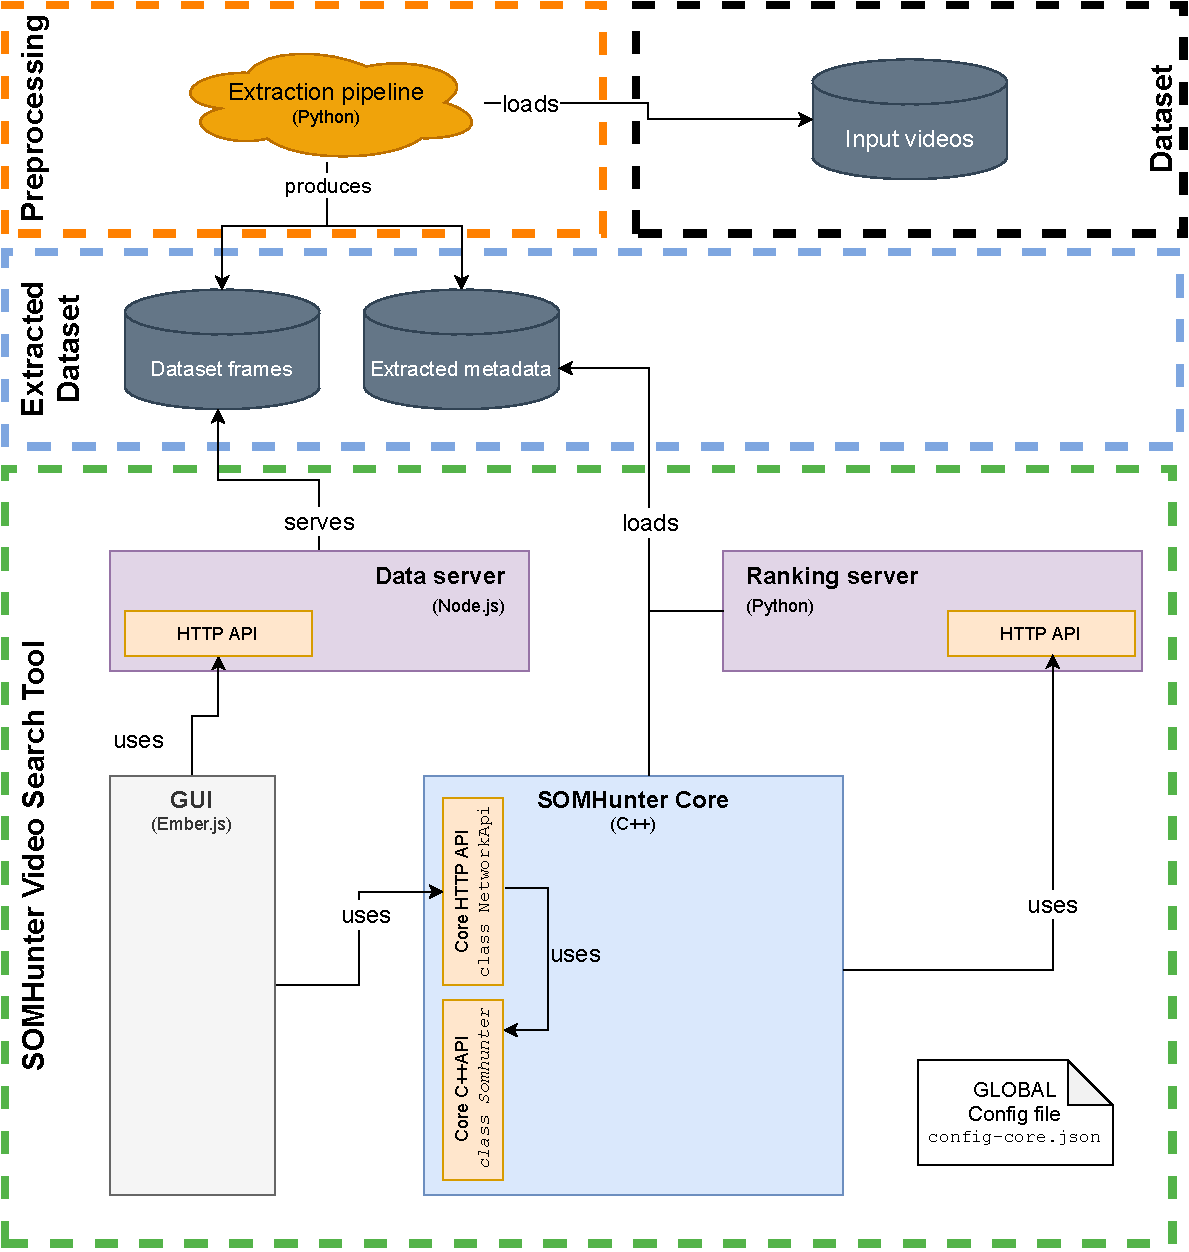
\includegraphics[width=1.0\textwidth]{img/diagrams/sh-arch.pdf}
	\caption{\textbf{High-level architecture of the SOMHunter tool.} Showing also extraction pipeline and visualising the path of the input dataset.}
	\label{fig:sh-arch}
\end{figure}

\section{Core}

The core is a stand-alone C++ piece of software that does all the hard work related to the search. In short, every search is represented and managed inside the core. The core is the director of everything here and the remaining components are just stateless services or helpers.

It loads the extracted dataset and holds the state of the ongoing search. It does all the query scoring, generates displays, handles all the logging and optionally communicates with a remote evaluation server (usually during the competitions). Every time a user does something, the core is notified either through C++ or HTTP API and it changes its state accordingly. 

More details about the core can be found in~\cref{comp-core}.

\section{UI}

The separation of the UI from the Core library gives us a wide range of possibilities such as trying new UI without a change of the Core functions, creating a restricted environment for experimental evaluations or using Core only as a backend service in a bigger environment. 

The UI component is a single page application written in the JavaScript framework Ember.js. Each UI fragment is an ember component and the event-driven architecture facilitates their communication. These components consist of a template and a JavaScript file defining its behaviour. The next layer is an action manager. It is a service that can be called from the components to facilitate communication with the Core. 

More on that in~\cref{comp-ui}.

\section{Data Server}

Over the years we concluded that the frames from the dataset are hard drive intensive and their size can grow in the future. Therefore this component provides an opportunity to move these frames on a remote server, where the frames may be saved and requested on demand. 

Our implementation is rather simple yet efficient. It is a node.js server that serves the data directory read from the core config.

\section{Ranking Server}

The latest trends in content-based video retrieval show us the importance of deep learning models employment. These models usually provide some semantic similarity rankings which are necessary for successful searches. Unfortunately, these models may require a different runtime environment such as programming language, framework or hardware demands (e.g. GPUs). On top of that, it is crucial to keep up with the newest versions to achieve state-of-the-art performance. Therefore we separated the main ranking into a single component that implements a simple API and takes care of the necessities described before.

More on that in~\cref{comp-ranking-server}.


\section{Other Component}
As we mentioned earlier, besides the tool itself there are other parts that are essential for the tool.

\subsection{Extraction Pipeline}

The extraction pipeline is an offline component. It takes the videos from the dataset and selects representative frames from them. The boundary detection models are employed to cut videos into the scenes from which we select only some frames to reduce redundancy. Then image metadata are extracted from these selected frames. In the end, the pipeline creates directories with selected frames and extracted features that can be loaded to SOMHunter.

More on that in~\cref{extraction-pipeline}.

\subsection{Extracted Dataset}

The extracted dataset consists of selected representative frames and their thumbnail version, the frame features for computing image similarity, the frame and text features for computing text to image similarity, and optionally date and hour attributes.

More on that in~\cref{extracted-dataset}.

\subsection{SOMCollector}

The creation of this standalone component was motivated by collecting user interaction logs in a restricted user environment to enhance the relevance feedback algorithm. It is a forked version from the open-source version of SOMHunter. Additionally, there were employed game elements. They made the interaction log collection more thrilling and motivated subjects to interact with the system a little longer. There is no longer an active development on this component to preserve the same environment for reproducibility sake.

More on that in~\cref{somcollector}.

\subsection{SOMHunter Simulator}

The interactive scoring part of the SOMHunter is the Bayesian relevance feedback algorithm. A disadvantage of an interactive algorithm is its exhausting optimization. It is mainly because every iteration of an interactive algorithm step needs a human user. The original algorithm has some parameters and if they are not set up properly, the algorithm won't produce a satisfactory result. So we would need to try many interactive searches to optimise the algorithm to sufficient settings. In this component, we mimic the user based on real-world data and provide a framework for prototyping interactive relevance feedback algorithms.

More on that in~\cref{somhunter-simulator}.


